\documentclass[11pt,fleqn]{exam}
\usepackage[utf8]{inputenc}

\usepackage[margin=1in]{geometry}
\usepackage{amsmath,amssymb}
\usepackage{gensymb}
\usepackage{marvosym}
\usepackage{multicol}
\usepackage{float}
\usepackage{graphicx}
\usepackage{units,icomma}
\usepackage[bahasa]{babel}
\usepackage[colorlinks,linkcolor=blue,urlcolor=blue]{hyperref}
\usepackage[margin=1.5cm]{caption}
\usepackage{wasysym}
\usepackage{tikzsymbols}
\usepackage[shortlabels]{enumitem}

\hyphenation{
  chro-no-ampe-ro-met-ric
  ber-dia-me-ter
  de-ngan
  meng-alam-i
  me-nem-pati
  mic-ro-graphs
  man-hat-tan-henge
  hi-tung-lah}

\addto\extrasbahasa{
	\def\figureautorefname{Gambar}
}

\renewcommand{\figurename}{Gambar.}
\def\equationautorefname{Persamaan}
\newcommand{\class}{OLIMPIADE ASTRONOMI}
\newcommand{\term}{Tingkat Provinsi - 2022}
\newcommand{\examnum}{OSP Astronomi 2022}
%\newcommand{\examdate}{11/02/2014}
%\newcommand{\timelimit}{120 Minutes}

%%%%%%%%% Units and Symbols
\newcommand*{\kms}{km s\ensuremath{^{-1}}}
\newcommand*{\Msun}{\ensuremath{M_{\odot}}}
\newcommand*{\Lsun}{\ensuremath{L_{\odot}}}
\newcommand*{\Rsun}{\ensuremath{R_{\odot}}}
\newcommand*{\Mstar}{\ensuremath{M_{\star}}}
\newcommand*{\Lstar}{\ensuremath{L_{\star}}}
\newcommand*{\Rstar}{\ensuremath{R_{\star}}}

\newcommand*{\jam}{\ensuremath{^{j}}}
\newcommand*{\h}{\ensuremath{^{h}}}
\newcommand*{\m}{\ensuremath{^{m}}}
\newcommand*{\s}{\ensuremath{^{s}}}
\newcommand*{\de}{\ensuremath{^{\circ}}}
\newcommand*{\am}{'}
\newcommand*{\as}{''}

\newcommand*{\alp}{\ensuremath{\alpha}}
\newcommand*{\del}{\ensuremath{\delta}}


\pagestyle{head}
\firstpageheader{}{}{}
\runningheader{\examnum}{}{Halaman \thepage\ dari \numpages}
\runningheadrule


\begin{document}

\noindent
\begin{tabular*}{\textwidth}{l @{\extracolsep{\fill}} r @{\extracolsep{6pt}} l}
\textbf{\class} \\% & \textbf{Name:} & \makebox[2in]{\hrulefill}\\
\textbf{\term}  %&&\\
%\textbf{\examnum} &&\\
%\textbf{\examdate} &&\\
%\textbf{Time Limit: \timelimit} & Teaching Assistant & \makebox[2in]{\hrulefill}
\end{tabular*}\\
\rule[2ex]{\textwidth}{2pt}

\noindent
\begin{tabular}{ll}
Copyright (c) 2023 & Ridlo W. Wibowo (ridloww@gmail.com)\\
                   & Sulistiyowati (sulis.astro08@gmail.com)
\end{tabular}

\vspace{0.3cm}
\noindent
Solusi ini dibuat tanpa jaminan kesesuaian dengan solusi resmi dari juri olimpiade sains bidang Astronomi. Pengguna boleh menyebarluaskan dan/atau memodifikasi solusi ini dengan mencantumkan sumber asli. Hak cipta soal ada pada Kemendiknas dan dilindungi undang-undang. Jika ada kesalahan jawaban/penulisan harap melaporkan ke alamat surel di atas.

\vspace{0.4cm}
\noindent
\rule[2ex]{\textwidth}{1.5pt}

% \textbf{Soal Pilihan Ganda}
\bigskip
\begin{questions}

\question Seorang pelaut yang menjelajah dengan kapalnya, memiliki kesempatan untuk mengamati fase-fase yang berbeda dari Bulan.

\begin{figure}[H]
\centering
\includegraphics[width=0.7\textwidth]{osp2022_1a.png}
\includegraphics[width=0.7\textwidth]{osp2022_1b.png}
%\caption{Foto asli rasi Crux. Oleh Eckhard Slawik.}
\label{fig:osp2022_1}
\end{figure}

Sepanjang malam dari 7 ke 8 November, posisi Bulan relatif terhadap sistem acuan Bumi Matahari adalah

\begin{choices}
\choice A
\choice B
\choice C
\choice D
\choice N
\end{choices}

\bigskip
\textit{Jawaban: } A

Dapat dilihat di gambar bahwa pengamatan untuk tanggal 7 ke 8 November bersesuaian dengan gambar paling kiri di barisan gambar pertama. Tertulis pengamatan dilakukan di bujur $10\degree$ BB (sekitar UTC-1) dan pengamatan dilakukan ketika pukul 11 malam waktu UTC, atau dalam waktu lokal sekitar pukul 10 malam. Gambar pada baris kedua menunjukkan bahwa fase bulan yang diamati saat itu adalah fase setengah (kuartir). Fase setengah yang mungkin diamati pukul 10 malam adalah fase kuartir pertama (posisi A), bukan fase kuartir ketiga (D) yang hanya bisa diamati setelah lewat tengah malam. 


\vspace{0.5cm}
\question Mengapa terdapat lebih sedikit kawah pada permukaan planet Venus, Bumi, dan Mars dibandingkan dengan pada permukaan Bulan atau Merkurius?
\begin{choices}
\choice Karena lebih sedikit meteorit yang menumbuk planet-planet tersebut
\choice Karena berhubungan dengan vulkanisme yang meregenerasi permukaan planet
\choice Karena Bumi dilindungi oleh Bulan
\choice Akibat dari erosi dan aberasi
\choice Karena struktur planet terrestrial yang didominasi gas dan cair
\end{choices}

\bigskip
\textit{Jawaban: } B atau D (kunci D)
\begin{itemize}
    \item Jumlah asteroid yang menumbuk planet tersebut bisa jadi lebih banyak karena luas permukaan dan kekuatan gravitasi yang lebih besar. (\textbf{Pilihan A Salah})
    \item Aktivitas vulkanisme di Venus, Bumi, dan Mars menjadi salah satu penyebab lebih cepat ``hilang''nya kawah bekas tumbukan, terutama saat masa awal planet dan Tata Surya terbentuk. (\textbf{Pilihan B Benar})
    \item Bulan memang menjadi pelindung Bumi, tetapi jumlah tumbukan ke Bumi akan tetap jauh lebih banyak, sehingga tidak secara lengkap menjelaskan lebih sedikitnya kawah di Bumi, apalagi kawah di Mars dan Venus. (\textbf{Pilihan C Salah})
    \item Erosi dan \textbf{abrasi} menjadi penyebab ``hilang''nya kawah di planet Bumi, Venus, dan Mars. (\textbf{Pilihan D Benar} dengan syarat kata aberasi diganti abrasi; dua kata ini sama-sama ada di KBBI, tetapi memiliki makna sangat berbeda)
    \item Struktur planet terestrial tidak didominasi gas dan cair. (\textbf{Pilihan E Salah})
\end{itemize}


\vspace{0.5cm}
\question Pernyataan di bawah ini yang SALAH jika dikaitkan dengan apa yang diperoleh dari spektrum  objek astronomi
\begin{choices}
\choice Temperatur ditentukan dari panjang gelombang puncak spektrum
\choice Komposisi kimia ditentukan dari kehadiran garis-garis spektral
\choice Laju pergerakan objek ditentukan dari posisi garis spektral
\choice Kehadiran gas lebih dingin diketahui dari kehadiran garis absorpsi pada spektrum
\choice Periode orbit objek ditentukan dari bentuk kontinum pada spektrum
\end{choices}

\bigskip
\textit{Jawaban: } E

Semua pernyataan benar kecuali pernyataan E, garis kontinum tidak dapat memberikan informasi mengenai periode orbit benda. 


\vspace{0.5cm}
\question Kalender Candra Kala Sunda adalah salah satu contoh kalender rembulan (\textit{lunar calendar}) di Nusantara yang menggunakan pola perulangan 8 tahunan (windu). Menurut suatu referensi, tahun kabisat kalender ini jatuh pada tahun ke-2, 4, 5, 6, dan 8 pada setiap pola perulangan windu tersebut. Dengan pola ini, sebagai contoh, tahun $t = 4$ dan tahun $t = 20$ keduanya adalah tahun kabisat. Tahun $t$ adalah kabisat jika
\begin{choices}
\choice sisa bagi dari pembagian $(2 + 3t)/8$ kurang dari 3
\choice sisa bagi dari pembagian $(2 + 3t)/8$ lebih dari 3
\choice sisa bagi dari pembagian $(5t - 1)/8$ adalah bilangan ganjil atau nol
\choice sisa bagi dari pembagian $(5t - 1)/8$ adalah bilangan genap atau nol
\choice sisa bagi dari pembagian $(5t - 1)/8$ adalah nol
\end{choices}

\bigskip
\textit{Jawaban: } C

Tahun kabisat pada kalender ini jatuh pada tahun ke-2, 4, 5, 6, dan 8 dengan siklus 8 tahunan; artinya ketika suatu tahun kabisat $t$ dibagi 8, sisa hasil pembagiannya  (modulo) adalah angka-angka tersebut: angka genap $\{0, 2, 4, 6 \}$ atau angka $\{5\}$, maka tahun $t$ tersebut adalah tahun kabisat.

Jika dinyatakan dalam persamaan lain, (2 + 3t), maka tahun kabisat akan terjadi ketika sisa hasil bagi/modulonya adalah $\{0, 1, 2, 4, 6\}$. 

Ketika dinyatakan dalam persamaan lain (5t - 1), maka tahun kabisat akan terjadi ketika sisa hasil bagi/modulonya adalah $\{0, 1, 3, 5, 7\}$.


\vspace{0.5cm}
\question Di suatu bagian dalam bintang, prosentase jumlah atom Hidrogen dan Helium masing-masing adalah 50 persen. Separuh dari seluruh Hidrogen kemudian mengalami ionisasi sempurna, dan separuhnya tetap dalam keadaan netral (tidak terionisasi). Demikian pula untuk Helium, separuh dari seluruh Helium juga kemudian mengalami ionisasi sempurna, dan separuhnya tetap dalam keadaan netral (tidak terionisasi). Akibat ionisasi ini, maka massa rata-rata partikel (menggunakan istilah baku berat molekul rata-rata) yang dinyatakan dalam massa atom Hidrogen ($m_H$) adalah
\begin{choices}
\choice $\frac{1+1+4+4}{1+2+1+3} = \frac{10}{7}$
\choice $\frac{1 \times 1 + 2 \times 1 + 1 \times 4 + 3 \times 4}{1+2+1+3} = \frac{19}{7}$
\choice $\frac{1 \times 1 + 2 \times 1 + 1 \times 4 + 3 \times 4}{1+1+4+4} = \frac{19}{10}$
\choice $\frac{1+2+1+3}{1+1+4+4} = \frac{7}{10}$
\choice Tidak dapat dihitung
\end{choices}

\bigskip
\textit{Jawaban: } A

Kita dapat asumsikan massa proton dan neutron hampir sama $m_p \approx m_n = m$ sedangkan massa elektron $m_e$ terlalu kecil dibanding massa proton dan neutron sehingga tidak menyumbang massa atom ($m_e \approx 0$). Jika jumlah atom Hidrogen ($^{1}_{1}$H) dan Helium ($^4_1$He) masing-masing 50\% dari total jumlah atom ($N$), maka massa total atom adalah 
$$M = \frac{1}{2} N \cdot m + \frac{1}{2} N \cdot 4 m = \frac{5}{2} N m$$
Jika di dalam bintang setengah dari Hidrogen dan Helium masing-masing terionisasi sempurna, maka jumlah partikel menjadi
\begin{eqnarray*}
    N_{\text{par}} &=& N_\text{H netral} + N_\text{H terionisasi sempurna} + N_\text{He netral} + N_\text{He terionisasi sempurna}\\
    N_{\text{par}} &=& \frac{1}{2} \cdot \frac{1}{2} N + 2 \cdot \frac{1}{2} \cdot \frac{1}{2} N + \frac{1}{2} \cdot \frac{1}{2} N + 3 \cdot \frac{1}{2} \cdot \frac{1}{2} N \\
    N_{\text{par}} &=& \left(\frac{1}{4} + \frac{1}{2} + \frac{1}{4} + \frac{3}{4}\right) N = \frac{7}{4} N 
\end{eqnarray*}

Massa rerata partikel menjadi
\begin{eqnarray*}
    \overline{m} &=& \frac{M}{N_{\text{par}}}\\
    \overline{m} &=& \frac{\frac{5}{2} N m}{\frac{7}{4} N}\\
    \overline{m} &=& \frac{10}{7} m 
\end{eqnarray*}


\vspace{0.5cm}
\question Pada gambar di bawah ini diberikan posisi empat buah objek yang mengorbit di sekitar pusat massa yang sama (arah gerak keempat objek sama). Orbit objek A dan B adalah lingkaran, sedangkan orbit objek C dan D adalah elips. Urutkan objek A, B, C, dan D dalam urutan kecepatan linier yang semakin besar.
\begin{figure}[H]
\centering
\includegraphics[width=0.5\textwidth]{osp2022_6.png}
\label{fig:osp2022_6}
\end{figure}

\begin{choices}
\choice A, B, C, D
\choice D, C, B, A
\choice C, A, D, B
\choice D, B, A, C
\choice B, D, A, C
\end{choices}

\bigskip
\textit{Jawaban: } D

Pada gambar dapat dilihat lingkaran-lingkaran konsentris dengan jarak teratur. Orbit A memiliki radius orbit 1 satuan, orbit B memiliki radius orbit 4 satuan, sedangkan orbit C dan D memiliki semimayor 2 satuan. Jika satuan panjang ini kita nyatakan dalam $a$, maka $a_A = a$, $a_B = 4a$, $a_C = a_D = 2a$.

Kecepatan orbit menjadi:
\begin{eqnarray*}
    v_A &=& \sqrt{\frac{GM}{a}}\\
    v_B &=& \sqrt{\frac{GM}{4a}}\\
    v_C &=& \sqrt{GM \left( \frac{2}{a} - \frac{1}{2a} \right)} = \sqrt{\frac{3GM}{2a}} \\
    v_D &=& \sqrt{GM \left( \frac{2}{3a} - \frac{1}{2a} \right)} = \sqrt{\frac{GM}{6a}}
\end{eqnarray*}
Dapat disimpulkan bahwa $v_D < v_B < v_A < v_C$


\vspace{0.5cm}
\question Dalam sebuah survei galaksi, terdapat 30 buah sampel galaksi yang diamati dan diukur jaraknya. Ternyata ditemukan bahwa sebagian besar galaksi berada pada suatu gugus galaksi  yang sama, dan sejumlah kecil galaksi ditemukan jaraknya secara signifikan lebih jauh dari gugus. Manakah dari besaran statistik di bawah ini yang dapat memberikan petunjuk jarak ke gugus tersebut jika kita menghitung semua sampel galaksi. 
\begin{choices}
\choice Rata-rata
\choice Median
\choice Modus
\choice Standar Deviasi
\choice Variansi
\end{choices}

\bigskip
\textit{Jawaban: } B

Jika kita libatkan galaksi yang jaraknya secara signifikan lebih jauh ke dalam perhitungan, maka secara statistik ``lebih aman'' jika kita gunakan median untuk menentukan jarak kita ke gugus galaksi. Nilai rata-rata bisa digunakan, tetapi nilai rata-rata umumnya lebih tidak aman terhadap data pencilan yang nilainya besar, karena data pencilan tersebut akan memiliki bobot lebih besar dalam perhitungan rata-rata. Secara statistik untuk jumlah data yang sedikit lebih aman menggunakan median dibanding nilai rata-rata untuk menggambarkan pusat sebaran data. 

Misalkan saja terdapat set data seperti berikut:
$\{3, 4, 5, 4, 3, 4, 30\}$, nilai rerata dari set data tersebut adalah 7.6, sedangkan mediannya adalah 4. Dapat dilihat bahwa nilai median lebih menggambarkan jarak ke \textit{cluster} data, sedangkan nilai rata-rata bergeser dari \textit{cluster} karena ada data pencilan 30 di dalamnya.  


\vspace{0.5cm}
\question Karena posisi Merkurius yang dekat dengan Matahari, planet ini mempunyai inti besi di pusatnya yang berukuran besar dan padat dibandingkan dengan bagian luar inti. Inti besi Merkurius mencapai 40\% dari volume Merkurius dan 60\% dari massa total Merkurius. Gunakan besaran-besaran berikut: Jari-jari Merkurius = 2440 km, Massa Merkurius = $3,3 \times 10^{23}$ kg. Dengan komposisi seperti ini, maka rapat massa rata-rata dari lapisan luar yang berupa batuan adalah
\begin{choices}
\choice $5,43 \times 10^{3}$ kg m$^{-3}$
\choice $3,35 \times 10^{10}$ kg m$^{-3}$
\choice $1,32 \times 10^{10}$ kg m$^{-3}$
\choice $3,62 \times 10^{3}$ kg m$^{-3}$
\choice $6,08 \times 10^{3}$ kg m$^{-3}$
\end{choices}

\bigskip
\textit{Jawaban: } D

Rapat massa lapisan luar Merkurius,
\begin{eqnarray*}
    \rho &=& \frac{M_\text{luar}}{V_\text{luar}}\\
    \rho &=& \frac{0,4 M_\text{Merkurius}}{0,6 V_\text{Merkurius}}\\
    \rho &=& \frac{0,4 \cdot 3,3\times 10^{23}}{0,6 \cdot \frac{4}{3} \pi (2440000)^3}\\
    \rho &=& 3615,5 \quad \text{kg m}^{-3}
\end{eqnarray*}


\vspace{0.5cm}
\question Pada suatu waktu di tanggal 21 Agustus 2022, planet Mars teramati memiliki diameter sudut 9,2 detik busur. Gunakan besaran-besaran berikut: Jari-jari Mars = 3397 km, kecepatan cahaya = $2,99792458 \times 10^8$ m/s. Jika di permukaan Mars telah didaratkan kendaraan penjelajah yang kemudian mengirimkan radar ke pengamat di Bumi, maka waktu yang diperlukan sinyal tersebut untuk sampai di Bumi adalah
\begin{choices}
\choice 246 detik
\choice 500 detik
\choice 193 detik
\choice 0,19 detik
\choice 0,5 detik
\end{choices}

\bigskip
\textit{Jawaban: } B

Jarak Mars saat itu dapat ditentukan dari diameter sudut dan diameter sebenarnya,
\begin{eqnarray*}
    d &=& \frac{2 \cdot 3397}{9,2 / 206265}\\
    d &=& 1,5232 \times 10^{8} \quad \text{km}
\end{eqnarray*}
Waktu yang dibutuhkan sinyal untuk sampai ke Bumi, 
\begin{eqnarray*}
    t &=& \frac{d}{c}\\
    t &=& \frac{1,5232 \times 10^{8}}{3 \times 10^5}\\
    t &=& 507,7 \quad \text{detik}
\end{eqnarray*}

\vspace{0.5cm}
\question Sebuah bintang bermassa 0,7 kali massa Matahari memiliki planet bermassa 1,6 kali massa Bumi yang mengorbit dengan periode 0,0022 tahun dan inklinasi 90 derajat. Gunakan besaran-besaran berikut: massa Matahari = $1,989 \times 10^{30}$ kg, massa Bumi = $5,97 \times 10^{24}$ kg. Jarak setengah sumbu panjang orbit planet adalah $2,7 \times 10^6$ km. Kecepatan radial bintang ini adalah

\begin{choices}
\choice $5,28 \times 10^7$ ms$^{-1}$
\choice $3,56 \times 10^{10}$ ms$^{-1}$
\choice $2,44 \times 10^5$ ms$^{-1}$
\choice $7,7$ ms$^{-1}$
\choice $1,7$ ms$^{-1}$
\end{choices}

\bigskip
\textit{Jawaban: } E

Kecepatan radial bintang yang dimaksud di soal sepertinya adalah kecepatan radial maksimum bintang ketika mengorbit pusat massa sistem (akibat tarikan gravitasi planet).

Hubungan pusat massa
\begin{eqnarray*}
    \frac{m_\text{p}}{m_\star} = \frac{a_\star}{a_\text{p}} = \frac{v_\star}{v_\text{p}}
\end{eqnarray*}
Kecepatan bintang mengorbit pusat massa,
\begin{eqnarray*}
    v_\star &=& \frac{m_p}{m_\star} v_\text{p}\\
    v_\star &=& \frac{m_p}{m_\star} \frac{2 \pi a_\text{p}}{P}\\
    v_\star &=& \frac{1,6 \cdot 5,97 \times 10^{24}}{0,7 \cdot 1,989 \times 10^{30}} \cdot \frac{2 \cdot \pi \cdot 2,7 \times 10^9 }{(0,0022 \cdot 365,25 \cdot 24 \cdot 3600)}\\
    v_\star &=& 1,676 \quad \text{m/s}
\end{eqnarray*}

\vspace{0.5cm}
\question Sebuah nebula dengan komposisi seluruhnya atom hidrogen, mempunyai massa 150 kali massa Matahari dan diameter 2 tahun cahaya. Gunakan besaran-besaran berikut ini: massa Matahari $= 1,989 \times 10^{30}$ kg, massa 1 atom hidrogen = $1,6735 \times 10^{-27}$ kg. Jika diasumsikan nebula ini berbentuk bola, maka rapat jumlah atom hidrogen di nebula tersebut adalah
\begin{choices}
\choice $1,2 \times 10^{57}$ atom hidrogen/cm$^3$
\choice $1,8 \times 10^{59}$ atom hidrogen/cm$^3$
\choice $5 \times 10^{4}$  atom hidrogen/cm$^3$
\choice $3,5 \times 10^{4}$ atom hidrogen/cm$^3$
\choice $3 \times 10^{3}$  atom hidrogen/cm$^3$
\end{choices}

\bigskip
\textit{Jawaban: } C

Rapat jumlah atom Hidrogen dapat dicari dari jumlah total atom Hidrogen dan Volume yang ia tempati,
\begin{eqnarray*}
    n &=& \frac{N}{V}\\
    n &=& \frac{150 \cdot 1,989 \times 10^{30} / 1,6735 \times 10^{-27}}{\frac{4}{3} \pi (1 \times 9,46 \times 10^{17} \text{cm})^3}\\
    n &=& 50273 \quad \text{atom/cm}^3
\end{eqnarray*}

\vspace{0.5cm}
\question Tumbukan antar asteroid atau pecahan ekor komet menghasilkan debu yang berserakan di Tata Surya dan perlahan tertarik ke arah Matahari. Debu ini akan menghamburkan cahaya dan saat dini hari tampak sebagai cahaya zodiak (\textit{zodiacal light}) yang tersebar di langit. Astronom kemudian menghitung kecerlangan permukaan cahaya zodiak ini bila diamati dari permukaan Bumi setara dengan 60 kali kecerlangan permukaan bintang magnitudo 10 (kecerlangan permukaan adalah kecerlangan yang diperoleh jika suatu fluks cahaya disebar dalam area 1 derajat persegi). Berapakah kecerlangan total cahaya zodiak yang mengisi seluruh area langit di atas horison pengamat di Bumi?
\begin{choices}
\choice 0,05 magnitudo
\choice 5,2 magnitudo
\choice -5,2 magnitudo
\choice -0,05 magnitudo
\choice 4,36 magitudo
\end{choices}

\bigskip
\textit{Jawaban: } C

Magnitudo per derajat persegi dari \textit{zodiacal light} adalah 
\begin{eqnarray*}
    m_1 - m_2 &=& -2,5 \log{\frac{E_1}{E_2}}\\
    m_\text{zl} - 10 &=& -2,5 \log{60} \\
    m_\text{zl} &=& 5,5546 \quad \text{mag/derajat}^2\\
\end{eqnarray*}
Total kecerlangan \textit{zodiacal light} untuk seluruh langit di atas horizon (setengah bola) adalah,
\begin{eqnarray*}
    m_\text{zl total} - m_\text{zl} &=& -2,5 \log{\left( \frac{\text{luas setengah bola dalam derajat persegi}}{\text{1 derajat persegi}} \right)}\\
    m_\text{zl total} - 5,5546 &=&  -2,5 \log{\left( \frac{2 \pi \text{  steradian}}{1 ^{\circ^{2}}} \right)}\\
    m_\text{zl total} - 5,5546 &=&  -2,5 \log{\left( \frac{2 \pi (57,3^{\circ} \cdot 57,3^{\circ})}{1 ^{\circ^{2}}} \right)}\\
    m_\text{zl total} &=& 5,5546 -2,5 \log{20626,5} \\
    m_\text{zl total} &=& -5,23
\end{eqnarray*}

\vspace{0.5cm}
\question Irfan mengamati Jupiter dengan menggunakan teleskop (lihat Gambar A). Tanpa sengaja, teleskopnya tersenggol sehingga posisi Jupiter bergeser dari tempatnya semula (lihat gambar B). Untuk mengembalikan Jupiter ke posisi semula, Irfan harus menggerakkan teleskop ke arah RA positif sebesar 0 jam 0 menit 5 detik. Dari deskripsi tersebut, arah X pada gambar menunjukkan arah apa?
\begin{figure}[H]
\centering
\includegraphics[width=0.7\textwidth]{osp2022_13.png}
\label{fig:osp2022_13}
\end{figure}
\begin{choices}
\choice Timur
\choice Barat
\choice Utara
\choice Selatan
\choice Tidak dapat ditentukan
\end{choices}

\bigskip
\textit{Jawaban: } A

Sesuai petunjuk di soal, arah yang ditunjukkan panah X adalah arah gerak teleskop, yang dijelaskan juga sebagai arah RA positif. Nilai RA bertambah berlawanan dengan arah gerak harian bintang, artinya untuk langit di atas Horizon nilai RA bertambah ke arah Timur, sehingga dapat disimpulkan arah X adalah arah Timur.

\vspace{0.5cm}
\question Salah satu jenis radiasi yang dapat dideteksi oleh teleskop radio adalah \textit{microwave amplification by stimulated emission of radiation} (maser). Diketahui radiasi maser berasal dari jarak 2,3 kpc dan memiliki rapat fluks (\textit{flux density}) sebesar 103 Jy pada frekuensi 1 kHz. Jika sumber radio bersifat isotropik, berapakah daya sumber radio tersebut dalam watt? Gunakan kesetaraan 1 Jy $= 10^{-26}$ W m$^{-2}$ Hz$^{-1}$
\begin{choices}
\choice $6 \times 10^{20}$ Watt
\choice $5 \times 10^{20}$ Watt
\choice $2 \times 10^{60}$ Watt
\choice $2 \times 10^{50}$ Watt
\choice $6 \times 10^{10}$ Watt
\end{choices}

\bigskip
\textit{Jawaban: } mungkin A

Sepertinya soal ini diterjemahkan dari bahasa Inggris, tetapi ada pemilihan kata yang salah, yaitu kata \textbf{pada} di kalimat ``... sebesar 103 Jy \textbf{pada} frekuensi 1 kHz.'' Hal ini memiliki arti bahwa pengamatan radio dilakukan \textbf{pada} frekuensi 1 kHz (padahal tidak mungkin untuk mengamati objek langit dari landas Bumi di frekuensi ini karena terhalang ionosfer). Untuk dapat menjawab pertanyaan, perlu diketahui lebar frekuensi pengamatan (\textit{bandwidth}), sehingga penggunaan kata ``pada'' harusnya ``dengan lebar frekuensi pengamatan''. Dengan sedikit \textit{googling} kita bisa temukan dari mana \textit{referensi} soal ini:
\begin{figure}[H]
\centering
\includegraphics[width=0.7\textwidth]{soalradio.png}
\label{fig:osp2022_14}
\end{figure}

Total fluks yang kita terima dalam rentang frekuensi pengamatan,
\begin{equation*}
    S = S_\nu \Delta \nu= 103 \times 10^{-26} \times 10^3 Hz = 1,03 \times 10^{-21} \text{  Watt/m}^2    
\end{equation*}
Luminositas benda pada rentang frekuensi tersebut:
\begin{equation*}
    L = S \cdot 4 \pi d^2 = 1,03 \times 10^{-21} \cdot 4 \pi (2300 \cdot 206265 \cdot 1,496 \times 10^{11})^2 = 6,52 \times 10^{19} \text{  watt}
\end{equation*}

Oh tidak, sepertinya angka yang diketikkan pada soal juga salah \Smiley{}. Mungkin seharusnya $10^3$ Jy tetapi tertulis 103 Jy. Jika diganti menjadi $10^3$ Jy, maka hasil akhirnya akan sama dengan solusi di soal aslinya. Sehingga jawaban yang tepat kemungkinan adalah $6 \times 10^{20}$ watt, sesuai dengan kunci jawaban yang dituliskan di soal (dari GDrive TOASTI). 


\vspace{0.5cm}
\question Sepanjang malam 14 hingga 15 November, Bulan mencapai ketinggian 90$\degree$. Situasi ini
\begin{figure}[H]
\centering
\includegraphics[width=0.7\textwidth]{osp2022_1a.png}
\includegraphics[width=0.7\textwidth]{osp2022_1b.png}
\label{fig:osp2022_15}
\end{figure}
\begin{enumerate}
    \item hanya dapat disaksikan ketika seseorang berada di sekitar garis khatulistiwa
    \item hanya mungkin ketika Bulan Purnama
    \item hanya mungkin terjadi dimana saja di permukaan Bumi setiap saat Bulan Purnama
    \item amat jarang dan paling banyak terjadi 2 kali dalam setahun untuk suatu lokasi
    \item tidak mungkin terjadi
\end{enumerate}

\bigskip
\textit{Jawaban: } 1, 4

Situasi Bulan melewati zenit (ketinggian 90\de) hanya mungkin terjadi untuk pengamat di lintang $-28,5^{\circ} < \phi < 28,5^{\circ}$. Deklinasi Bulan akan berubah dalam rentang tersebut dengan periode sekitar 27,4 hari, tetapi ketika nilai deklinasi Bulan sama dengan lintang pengamat, saat itu pengamat belum tentu tepat di bawahnya (karena Bumi memiliki rotasi dengan periodenya sendiri), sehingga kejadian Bulan melewati zenit pengamat tidak terjadi 2 kali tiap bulannya. Situasi ini juga dapat terjadi pada fase apa saja. 

\vspace{0.5cm}
\question Ketika sebuah komet berada jauh dari Matahari, maka melalui teleskop kita mengamatinya sebagai objek bola yang kecil, tetapi ketika mendekati Bumi, akan tampak memiliki koma dan ekor-ekor yang panjang. Manakah di antara pernyataan berikut ini yang BENAR?
\begin{enumerate}
\item Gaya gravitasi dari Matahari bertambah ketika komet mendekati dan ini akan meregangkan komet
\item Materi gelap yang tak terlihat sekitar Matahari akan memoles komet menjadi bentuk yang panjang
\item Materi yang bersifat volatil dari komet mulai menyublim, dan tekanan radiasi dan angin Matahari akan menyebabkan ekor komet terbentuk
\item Pembentukan ekor komet dan materi yang menyublim ditunjukkan oleh fakta bahwa ekor komet arahnya menjauh dari Matahari
\item Komet tersusun atas material stoney-iron yang kompak
\end{enumerate}

\bigskip
\textit{Jawaban: } 3, 4

\begin{itemize}
    \item Gaya gravitasi benar bertambah besar ketika komet mendekati, tapi gaya gravitasi saja tidak meregangkan komet. Gradien gaya gravitasi (gaya pasang surut) yang dirasakan kometlah yang dapat menjelaskan peregangan badan komet. (Pernyataan 1 Salah)
    \item Materi gelap (\textit{dark matter}) memang ada di Tata Surya dan sekitar kita, tetapi tidak dominan pengaruhnya terhadap perubahan fisis komet. (Pernyataan 2 Salah)
    \item Komet umumnya tersusun dari kumpulan debu, es, dan bebatuan kecil yang menyatu. (Pernyataan 5 Salah)
\end{itemize}

\vspace{0.5cm}
\question Gambar berikut adalah skema dasar penentuan jarak geosentris dari Bumi (berpusat di $E$) ke suatu kawah $M$ di Bulan oleh seorang pengamat di titik $A$ di permukaan Bumi, yang dengan disederhanakan dapat dianggap sebagai jarak perkiraan Bumi-Bulan. Sudut-sudut $\alpha$ dan $z$ diketahui atau diukur. Pada skema ini berlaku
\begin{figure}[H]
\centering
\includegraphics[width=0.7\textwidth]{osp2022_17.png}
\label{fig:osp2022_17}
\end{figure}
\begin{enumerate}
\item Lintang untuk $A$ adalah sebesar $z$ derajat
\item Meridian untuk $A$ adalah sebesar $p$ derajat diukur ke Timur dari kota Greenwich
\item Berlaku persamaan $p + z = 180^{\circ} - \alpha$
\item Bila radius Bumi adalah EA$ = r$, maka jarak EM$ = r\sin{\alpha}/\sin{(\alpha - z)}$
\item Jarak AM dapat dihitung
\end{enumerate}

\bigskip
\textit{Jawaban: } 1, 4, 5

\begin{itemize}
\item Lintang untuk $A$ adalah sebesar $z$ derajat, hal ini dapat dilihat langsung di gambar. (Pernyataan 1 Benar)
\item Sudut $p$ tidak menyatakan bujur atau meridian pengamat. (Pernyataan 2 Salah)
\item Dapat dianalisis dari sudut luar segitiga, maka berlaku persamaan $p + z = \alpha$. (Pernyataan 3 Salah)
\item Dari segitiga di soal dapat ditulis hubungan sinus,
\begin{eqnarray*}
    \frac{\text{EM}}{\sin(180^{\circ}-\alpha)} &=& \frac{\text{EA}}{\sin{p}}\\
    \frac{\text{EM}}{\sin{\alpha}} &=& \frac{r}{\sin{p}}\\
    \text{EM} &=& \frac{r \sin{\alpha} }{\sin{(\alpha - z)}}
\end{eqnarray*}
(Pernyataan 4 Benar)
\item Jarak AM dapat dihitung, kenapa tidak? (Pernyataan 5 Benar)
\end{itemize}

\vspace{0.5cm}
\question Nilai $\gamma$ yang ada pada gambar berikut adalah jarak dari sumbu kerucut bayangan Bulan (garis putus-putus) ke pusat Bumi dibagi dengan nilai radius Bumi. Besaran $\gamma$ ini muncul pada data perkiraan gerhana, termasuk yang akan terjadi pada gerhana Matahari hybrid 20 April 2023 yang melewati wilayah Indonesia.
\begin{figure}[H]
\centering
\includegraphics[width=0.5\textwidth]{osp2022_18.png}
\label{fig:osp2022_18}
\end{figure}
\begin{enumerate}
\item Kerucut bayangan yang dimaksud hanya untuk umbra, tidak untuk penumbra
\item Puncak kerucut bayangan dapat mengarah ke Utara atau Selatan
\item Mungkin saja berlaku $\gamma > 1$
\item Rentang nilai $\gamma$ adalah $0 < \gamma < 1$
\item Perhitungan $\gamma$ juga dapat dilakukan untuk peristiwa gerhana Bulan
\end{enumerate}

\bigskip
\textit{Jawaban: } 2, 3, 5

\begin{itemize}
    \item Kerucut umbra dan penumbra memiliki pusat/puncak yang sama. (Pernyataan 1 Salah)
    \item Bayangan Bulan dapat berada di belahan Bumi Utara dan Selatan tergantung posisi relatif Bulan terhadap kemiringan Bumi saat gerhana terjadi. (Pernyataan 2 Benar)
    \item Nilai gamma ($\gamma$) yang sering digunakan saat gerhana terjadi menggambarkan seberapa ``pusat'' atau seberapa jauh pusat bayangan benda satu terhadap benda lain yang digerhanai, jarak ini dinyatakan dalam radius Bumi di ekuator. (Pernyataan 3 dan 5 Benar)
\end{itemize}

\vspace{0.5cm}
\question Tabel di bawah ini menggambarkan contoh kemunculan garis-garis spektrum pada lima episode pekerjaan (\textit{batch}) analisis pola dan asosiasi garis-garis spektrum. Kebanyakan garis pada tabel adalah berasal dari unsur Hidrogen (mulai dari $H_{\alpha}$ hingga $H_{\epsilon}$) dan salah satu garis ion Kalsium (sering disebut garis $K$)
\begin{table}[H]
\centering
\begin{tabular}{| l | l |}
\hline
\textit{batch} & Kemunculan garis-garis spektrum \\
\hline
1              & $H_{\alpha}, H_{\beta}, H_{\gamma}$ \\
\hline
2              & $H_{\alpha}, H_{\delta}, H_{\gamma}$ \\
\hline
3              & $H_{\alpha}, H_{\gamma}, H_{\epsilon}$ \\
\hline
4              & $H_{\beta}, H_{\epsilon}, K$ \\
\hline
5              & $H_{\beta}, H_{\delta}, H_{\gamma}, H_{\epsilon}, K$\\
\hline
\end{tabular}
\end{table}
\begin{enumerate}
    \item Kemunculan pola  $H_{\alpha}$ dan $H_{\gamma}$ sering terjadi
    \item Jika $H_{\alpha}$ muncul, dipastikan $H_{\gamma}$ juga muncul
    \item Jika $H_{\gamma}$ muncul, dipastikan $H_{\alpha}$ juga muncul
    \item Tingkat kepastian asosiasi $H_{\alpha}$ disertai kemunculan $H_{\gamma}$ adalah 100\%
    \item Tingkat kepastian asosiasi $H_{\gamma}$ disertai kemunculan $H_{\alpha}$ adalah 75\%
\end{enumerate}

\bigskip
\textit{Jawaban: } 1, 2, 4, 5

\begin{itemize}
    \item Kemunculan pola  $H_{\alpha}$ dan $H_{\gamma}$ sering terjadi. Pernyataan ini mungkin  benar, tergantung definisi `sering' itu apa. (Pernyataan 1 Benar)
    \item Jika $H_{\alpha}$ muncul, dipastikan $H_{\gamma}$ juga muncul; sesuai dengan tabel ketika ada $H_{\alpha}$ maka muncul juga $H_{\gamma}$ (Pernyataan 2 Benar)
    \item Jika $H_{\gamma}$ muncul, dipastikan $H_{\alpha}$ juga muncul; tidak sesuai untuk \textit{batch} 5. (Pernyataan 3 Salah)
    \item Tingkat kepastian asosiasi $H_{\alpha}$ disertai kemunculan $H_{\gamma}$ adalah 100\%; sesuai dengan data, 3 dari 3 \textit{batch} $H_{\alpha}$ disertai dengan kemunculan $H_{\gamma}$. (Pernyataan 4 Benar)
    \item Tingkat kepastian asosiasi $H_{\gamma}$ disertai kemunculan $H_{\alpha}$ adalah 75\%; sesuai dengan data, 3 dari 4 \textit{batch} kemunculan $H_{\gamma}$ disertai dengan kemunculan $H_{\alpha}$. (Pernyataan 5 Benar)
\end{itemize}

\vspace{0.5cm}
\question Metode penentuan jarak berikut ini yang TIDAK PERNAH digunakan oleh para astronom untuk mengukur jarak ke ekstragalaksi adalah
\begin{enumerate}
    \item Paralaks trigonometri
    \item Bintang variabel Cepheid
    \item Hukum Hubble
    \item Metode gerak gugus
    \item Supernova tipe Ia
\end{enumerate}

\bigskip
\textit{Jawaban: } 1, 4

Metode paralaks dan metode gerak gugus (\textit{moving cluster}) hanya dapat digunakan untuk menentukan jarak bintang dan gugus yang ada di dekat Matahari.


\vspace{0.5cm}
\question Di antara enam pernyataan di bawah ini, pernyataan yang BENAR adalah
\begin{enumerate}
    \item Galaksi tersebar merata di seluruh alam semesta
    \item Menurut prinsip kosmologis, dalam volume yang cukup besar, alam semesta akan terlihat kurang lebih sama di mana pun pengamat berada
    \item Struktur terbesar yang dapat diamati di alam semesta saat ini adalah \textit{supercluster}, rongga (\textit{void}), dan filamen
    \item Menurut prinsip kosmologis, jika pengamat melihat cukup jauh, maka alam semesta akan terlihat kurang lebih sama di semua arah
    \item Secara rata-rata, jumlah galaksi yang cahayanya tampak mengalami pergeseran merah sama banyaknya dengan jumlah galaksi yang mengalami pergeseran cahaya biru
    \item Atom-atom yang memancarkan foton \textit{Cosmic Microwave Background} (CMB) yang kita amati hari ini hanya berjarak 400 ribu tahun cahaya
\end{enumerate}

\bigskip
\textit{Jawaban: } 2, 3, 4

\begin{itemize}
    \item Galaksi tersebar merata di seluruh alam semesta (\textit{homogen}), kalau dilihat dalam skala besar. (Pernyataan 1 mungkin Salah)
    \item Galaksi yang jauh semuanya mengalami pergeseran merah (\textit{redshift}). (Pernyataan 5 Salah)
    \item Menurut model standar yang dipercaya saat ini, foton CMB berawal dari masa awal Alam Semesta. CMB merupakan cahaya pertama yang dipancarkan Alam Semesta (saat \textit{decoupling} dari materi) ketika usia alam semesta sekitar 380000 tahun setelah Big Bang. (Pernyataan 6 Salah)
\end{itemize}

\vspace{0.5cm}
\question Pada spektrum dari sebuah bintang (tunggal), teramati garis Oksigen pada 5012 \AA, dengan panjang gelombang diam pada 5007 \AA. Gerak diri bintang ini diamati sebesar 1 detik busur per tahun, dengan jarak bintang 60 parsek. Gunakan besaran kecepatan cahaya = $2,99792458 \times 10^8$ m/s. Kecepatan diri dan arah gerak bintang terhadap pengamat adalah
\begin{enumerate}
    \item 400 kms$^{-1}$
    \item 500 kms$^{-1}$
    \item 270 kms$^{-1}$
    \item Mendekati
    \item Menjauhi
    \item Mendekati kemudian menjauhi
    \item Menjauhi kemudian mendekati
\end{enumerate}

\bigskip
\textit{Jawaban: } 1, 5

Kecepatan radial bintang:
\begin{eqnarray*}
    \frac{v_r}{c} &=& \frac{\Delta \lambda}{\lambda_0}\\
    v_r &=& \frac{5}{5007} \cdot 3 \times 10^{5}\\
    v_r &=& 299,6 \text{  km/s (\textit{redshift} / menjauhi pengamat)}
\end{eqnarray*}
Kecepatan tangensial bintang:
\begin{eqnarray*}
    v_t &=& 4,74 \mu d\\
    v_t &=& 284.4 \text{  km/s}
\end{eqnarray*}
Kecepatan bintang:
\begin{eqnarray*}
    v &=& \sqrt{v_r^2 + v_t^2}\\
    v &=& 413 \text{  km/s}
\end{eqnarray*}

\vspace{0.5cm}
\question Elon Musk mengirimkan tim SpaceX untuk menjelajah Mars. Roket Falcon 9 yang mereka gunakan mendarat tepat di kutub utara Mars. Saat menengadah, mereka melihat penampakan langit di arah zenit seperti pada gambar berikut (zenit ditandai dengan +Z).
\begin{figure}[H]
\centering
\includegraphics[width=0.8\textwidth]{osp2022_23.png}
\label{fig:osp2022_23}
\end{figure}
Pilihlah pernyataan yang BENAR berdasarkan informasi di atas
\begin{enumerate}
    \item Seluruh bintang yang terlihat di gambar adalah bintang sirkumpolar
    \item Segitiga musim panas (\textit{summer triangle}) tidak teramati
    \item Bintang Polar di Mars adalah Polaris
    \item Galaksi Andromeda berada di atas horison
    \item Lintasan orbit Bumi akan berada dekat dengan zenith Mars, (kurang dari 5 derajat) karena kemiringan sumbu rotasi kedua planet hampir sama besar
    \item Di Mars tidak terjadi perubahan musim karena jaraknya terlalu jauh dari Matahari
\end{enumerate}

\bigskip
\textit{Jawaban: } 1, 4

\begin{itemize}
    \item Seluruh bintang yang terlihat di gambar adalah bintang sirkumpolar $\rightarrow$ Pernyataan ini benar karena dikatakan bahwa pengamat ada tepat di Kutub Utara Mars.
    \item Segitiga musim panas (\textit{summer triangle}) tidak teramati $\rightarrow$ Pernyataan ini tidak benar karena dapat kita kenali dengan mudah di peta langit yang diberikan ketiga bintang anggota \textit{summer triangle}: Deneb, Vega, dan Altair (tiga bintang terang di sisi kanan gambar)
    \item Bintang Polar di Mars adalah Polaris $\rightarrow$ Pernyataan ini salah karena posisi Kutub Langit Utara Mars seharusnya yang ditunjukkan pada titik Z di gambar, dan pada titik itu tidak ada bintang Polaris.
    \item Galaksi Andromeda berada di atas horison $\rightarrow$ Pernyataan yang benar, galaksi Andromeda dapat ditemukan di antara rasa Cassiopeia, Andromeda, dan Pegasus (di sisi bawah gambar).
    \item Lintasan orbit Bumi akan berada dekat dengan zenith Mars, (kurang dari 5 derajat) karena kemiringan sumbu rotasi kedua planet hampir sama besar $\rightarrow$ Pernyataan ini salah, karena kemiringan sumbu rotasi yang hampir sama malah menyebabkan tidak memungkinkan Bumi untuk lewat dekat zenit pengamat yang ada di Kutub Utara Mars.
    \item Di Mars tidak terjadi perubahan musim karena jaraknya terlalu jauh dari Matahari $\rightarrow$ Pernyataan ini salah, karena di Mars terjadi perubahan musim mirip dengan di Bumi karena kemiringan sumbu rotasi yang hampir sama (24\de)
\end{itemize}
\begin{figure}[H]
\centering
\includegraphics[width=0.8\textwidth]{osp2022_23_jawab.png}
\label{fig:osp2022_23_jawab}
\end{figure}

\vspace{0.5cm}
\question Jika mata manusia (diameter 24 mm dan panjang fokus lensa 17 mm) dibuat menjadi sebesar Teleskop James Webb (JWST) (diameter 6,5 m dan panjang fokus 131,4 m), maka pilihlah pernyataan yang BENAR di bawah ini
\begin{enumerate}
    \item Manusia di Bumi akan mampu melihat bendera selebar 1,5 meter yang ditancapkan Neil Armstrong di Bulan (berjarak 384,4 juta km dari Bumi)
    \item Matahari akan tampak 73 ribu kali lebih terang
    \item Manusia akan dapat melihat lingkungan sekitar dengan medan pandang yang lebih luas seperti mata lalat
    \item Langit malam akan terlihat terang seperti senja hari
    \item Manusia akan dapat melihat benda kecil di dekatnya dengan lebih jelas
    \item Bulan purnama akan terlihat lebih besar
\end{enumerate} 

\bigskip
\textit{Jawaban: } 2, 6

Besar sekali diameter (pupil) matanya, 24 mm?
\begin{itemize}
    \item Manusia di Bumi akan mampu melihat bendera selebar 1,5 meter yang ditancapkan Neil Armstrong di Bulan (berjarak 384,4 juta km dari Bumi) $\rightarrow$ jarak Bulan atau mungkin satuannya sudah salah; andaikan kita gunakan jarak yang benar, maka akan kita peroleh diameter sudut bendera adalah $3,9 \times 10^{-9}$ rad, sedangkan sudut terkecil yang dapat dipisahkan mata JWSTnya (asumsi melihat di visual, tidak di inframerah seperti JWST) adalah $\theta_\text{res} = \frac{1,22 \lambda}{D} = 1,03 \times 10^{-7}$ rad. Sehingga dapat disimpulkan bahwa resolusi mata JWST tidak cukup untuk dapat melihat/memisahkan bendera di Bulan.
    \item Matahari akan tampak 73 ribu kali lebih terang\\
    Tingkat kecerlangan objek langit berbanding lurus dengan luas area bukaan teleskop atau diameter kuadrat,
    \begin{eqnarray*}
        \text{rasio} = \left(\frac{6500}{24}\right)^2 = 73350
    \end{eqnarray*}
    $\rightarrow$ Pernyataan 2 Benar
    \item Manusia akan dapat melihat lingkungan sekitar dengan medan pandang yang lebih luas seperti mata lalat $\rightarrow$ Pernyataan ini salah karena medan pandang akan menyempit dengan panjang fokus yang lebih panjang.
    \item Langit malam akan terlihat terang seperti senja hari $\rightarrow$ tidak diberikan data kecerlangan langit (\textit{sky brightness}) senja yang dimaksud (kecerlangan senja itu sangat bervariasi, merentang dari saat Matahari terbenam hingga ketinggian $-18^{\circ}$); sepertinya pernyataan yang salah dan/atau tidak dapat diperiksa.
    \item Manusia akan dapat melihat benda kecil di dekatnya dengan lebih jelas $\rightarrow$ apa definisi ``lebih jelas'' di kalimat ini? teleskopnya diubah menjadi mikroskop? Sepertinya pernyataan yang salah karena teleskop pada umumnya tidak bisa melihat benda yang sangat dekat.
    \item Bulan purnama akan terlihat lebih besar $\rightarrow$ pernyataan ini benar karena medan pandang teleskop akan menjadi lebih sempit (perbesaran membesar).
\end{itemize}

\vspace{0.5cm}
\question Suatu malam, seorang pengamat melihat langit seperti pada gambar berikut.
\begin{figure}[H]
\centering
\includegraphics[width=0.8\textwidth]{osp2022_25.png}
\label{fig:osp2022_25}
\end{figure}
Pilihlah pernyataan yang BENAR.
\begin{enumerate}
    \item Ekliptika ditunjukkan oleh garis berwarna kuning
    \item Mars, Jupiter, dan Saturnus akan berada dekat dengan garis berwarna merah
    \item Pengamat tersebut berada di belahan Bumi utara
    \item Rasi bintang Gemini akan terbenam di Barat
    \item Pada malam itu, pengamat yang lahir tanggal 1 Mei dan memiliki zodiak Taurus, sedang berulang tahun
    \item Arah pusat galaksi Bima Sakti tidak tampak di gambar tersebut
\end{enumerate}

\bigskip
\textit{Jawaban: } 2, 3, 6

\begin{itemize}
    \item Rasi-rasi yang dilewati masing-masing garis menunjukkan bahwa garis merah merupakan lingkaran ekliptika langit (melewati zodiak dan planet-planet) sedangkan garis kuning adalah ekuator langit (melewati Orion) $\rightarrow$ Pernyataan 1 Salah, Pernyataan 2 Benar
    \item Rasi Ursa Minor, Draco, Cygnus dll yang ada di sisi atas gambar menunjukkan bahwa sisi atas adalah arah Utara langit. Polaris yang terlihat menunjukkan bahwa pengamat ada di belahan Bumi Utara.  (\textit{Northern hemisphere}) $\rightarrow$ Pernyataan 3 Benar
    \item Rasi Gemini\---dan bintang-bintang lain\---akan terbenam di sisi Barat langit, akan tapi Gemini tidak terbenam tepat di arah Barat; karena lokasinya tidak berada di ekuator langit. $\rightarrow$ Pernyataan 4 Salah
    \item Orang yang memiliki zodiak Taurus tidak berulang tahun di hari itu karena rasi Taurus terlihat di langit malam itu. Zodiak seseorang disesuaikan dengan rasi yang ada di belakang Matahari ketika dia lahir. $\rightarrow$ Pernyataan 5 Salah
    \item Pusat galaksi ada di arah rasi Sagitarius-Scorpio, yang letaknya berlawanan dengan rasi Aries dan Pisces yang ada di gambar tersebut. $\rightarrow$ Pernyataan 6 Benar
\end{itemize}


\vspace{1cm}
\textbf{SOAL ISIAN SINGKAT}

\vspace{0.5cm}
\question Andaikan kamu seorang astronom yang sedang menelaah sistem bintang ganda gerhana. Setelah mengamati sistem bintang ini secara spektroskopi selama beberapa tahun, sejumlah informasi berikut terkumpul:
\begin{enumerate}[a.]
    \item Periode orbit 2,63 tahun
    \item Bintang 1 memiliki kecepatan Doppler yang berubah antara +20,4 kms$^{-1}$ dan -20,4 kms$^{-1}$
    \item Bintang 2 memiliki kecepatan Doppler yang berubah antara +6,8 kms$^{-1}$ dan -6,8 kms$^{-1}$
    \item Kedua bintang berevolusi satu sama lain dalam bentuk orbit lingkaran
\end{enumerate}
Maka, radius orbit bintang 1 adalah $\ldots$ sa, dan bintang 2 adalah $\ldots $ sa, dan massa bintang 1 adalah $\ldots M_\odot$ dan bintang 2 adalah $\ldots M_\odot$.


\bigskip
\textit{Jawaban: } 1,8 ; 0,6 ; 0,5 ; 1,5 

\textit{Kunci: } 1.8 ; 0.6 ; 2.0 ; 1.5 (toleransi masing-masing 10\%)

Di soal disebutkan bahwa sistem bintang ganda ini adalah bintang ganda gerhana, yang artinya inklinasi orbitnya $\sim 90^{\circ}$, sehingga kecepatan radial maksimum yang diperoleh dari spektrum adalah kecepatan orbitnya.

Kecepatan orbit masing-masing bintang mengelilingi pusat massa adalah
\begin{eqnarray*}
    v_1 &=& \frac{2 \pi r_1}{P}\\
    v_2 &=& \frac{2 \pi r_2}{P}\\
\end{eqnarray*}
Radius orbit masing-masing bintang dapat dihitung dengan rumus di atas, menghasilkan nilai $r_1 = 1,8$ sa dan $r_2 = 0.6$ sa.

Massa sistem bintang dapat dihitung dengan,
\begin{eqnarray*}
    M_1 + M_2 &=& \frac{a^3}{P^2}\\
    M_1 + M_2 &=& \frac{(1,8 + 0.6)^3}{2,63^2}\\
    M_1 + M_2 &=& 2 M_\odot
\end{eqnarray*}
Dari hubungan pusat massa $M_1/M_2 = v_2/v_1 = r_2 / r_1 = 1/3$, dapat kita turunkan massa masing-masing bintang,
\begin{eqnarray*}
    \frac{1}{3} M_2 + M_2 &=& 2 M_\odot\\
    M_2 &=& 1,5 M_\odot\\
    M_1 &=& 0,5 M_\odot
\end{eqnarray*}

\vspace{0.5cm}
\question Di suatu kota, dengan lintang sebesar $L = 37,7^{\circ}$, sebuah bidang lingkaran seperti pada gambar telah disiapkan sebagai alat bantu untuk membangun jam Matahari (\textit{sundial}) yang menempel di dinding vertikal (\textit{vertical sundial}). Sebuah batang tegak lurus bidang lingkaran (\textit{gnomon}) juga telah dipasangkan dengan kuat. Diketahui jari-jari lingkaran tersebut adalah sebesar $a=1$. Angka-angka yang tercantum di bidang lingkaran telah didasarkan pada hasil pengamatan. Notasi W, E, N, dan S masing-masing adalah notasi titik kardinal Barat, Timur, Utara, dan Selatan.
\begin{figure}[H]
\centering
\includegraphics[width=0.6\textwidth]{osp2022_27.png}
\label{fig:osp2022_27}
\end{figure}
\begin{enumerate}[A.]
    \item Kota tersebut ada di wilayah Bumi bagian $\ldots$
    \item Jika lingkaran tersebut akan diproyeksikan di dinding (tegak), maka pada dinding harus digambarkan sebuah lonjongan (elips) dengan salah satu sumbu sepanjang $a=1$ meter, dan sumbu lain adalah sepanjang $b = \ldots $ meter (dinyatakan hingga 2 angka di kanan tanda pecahan desimal, dengan ejaan angka dalam bahasa Inggris)
    \item Untuk bidang lingkaran, pada saat jam 11 siang, sudut yang dibentuk terhadap posisi jam 12 adalah sebesar $T=15$ derajat, namun untuk bidang elips di dinding, sudut yang dibentuk terhadap posisi jam 12 siang adalah sebesar $H=\ldots$ derajat (tanpa angka di kanan tanda pecahan desimal)
\end{enumerate}

\bigskip
\textit{Jawaban: } SELATAN ; 1.26 ; 12

\begin{enumerate}[A.]
\item \textit{Vertical sundial} adalah salah satu jenis jam Matahari yang diletakkan di dinding, yang biasa digunakan untuk lintang tinggi ($> 23,5^{\circ}$). Hal penting yang perlu diperhatikan adalah gnomon \textit{vertical sundial}  harus tetap miring dan mengarah ke KLU dan KLS (lihat gnomon garis hijau pada gambar di bawah ini). 
\begin{figure}[H]
\centering
\includegraphics[width=0.3\textwidth]{VerticalSundial1.png}
\includegraphics[width=0.49\textwidth]{VerticalSundial.png}
\captionsetup{labelformat=empty}
\caption{Contoh \textit{vertical sundial} dan penjelasannya}
\label{fig:osp2022_27_jawab}
\end{figure}

Di gambar ditunjukkan bahwa (1) kemiringan gnomon dengan lantai sama dengan lintang pengamat $L = 37,7^{\circ}$, (2) elevasi gnomon sebesar lintang tersebut menghadap ke arah Selatan, (3) posisi gnomon tegak lurus papan lingkaran penerima bayangan gnomon; \textit{sundial} seperti ini bukan merupakan \textit{vertical sundial} melainkan \textit{equatorial sundial} untuk posisi pengamat di lintang $37,7^{\circ}$ LS (SELATAN).
\begin{figure}[H]
\centering
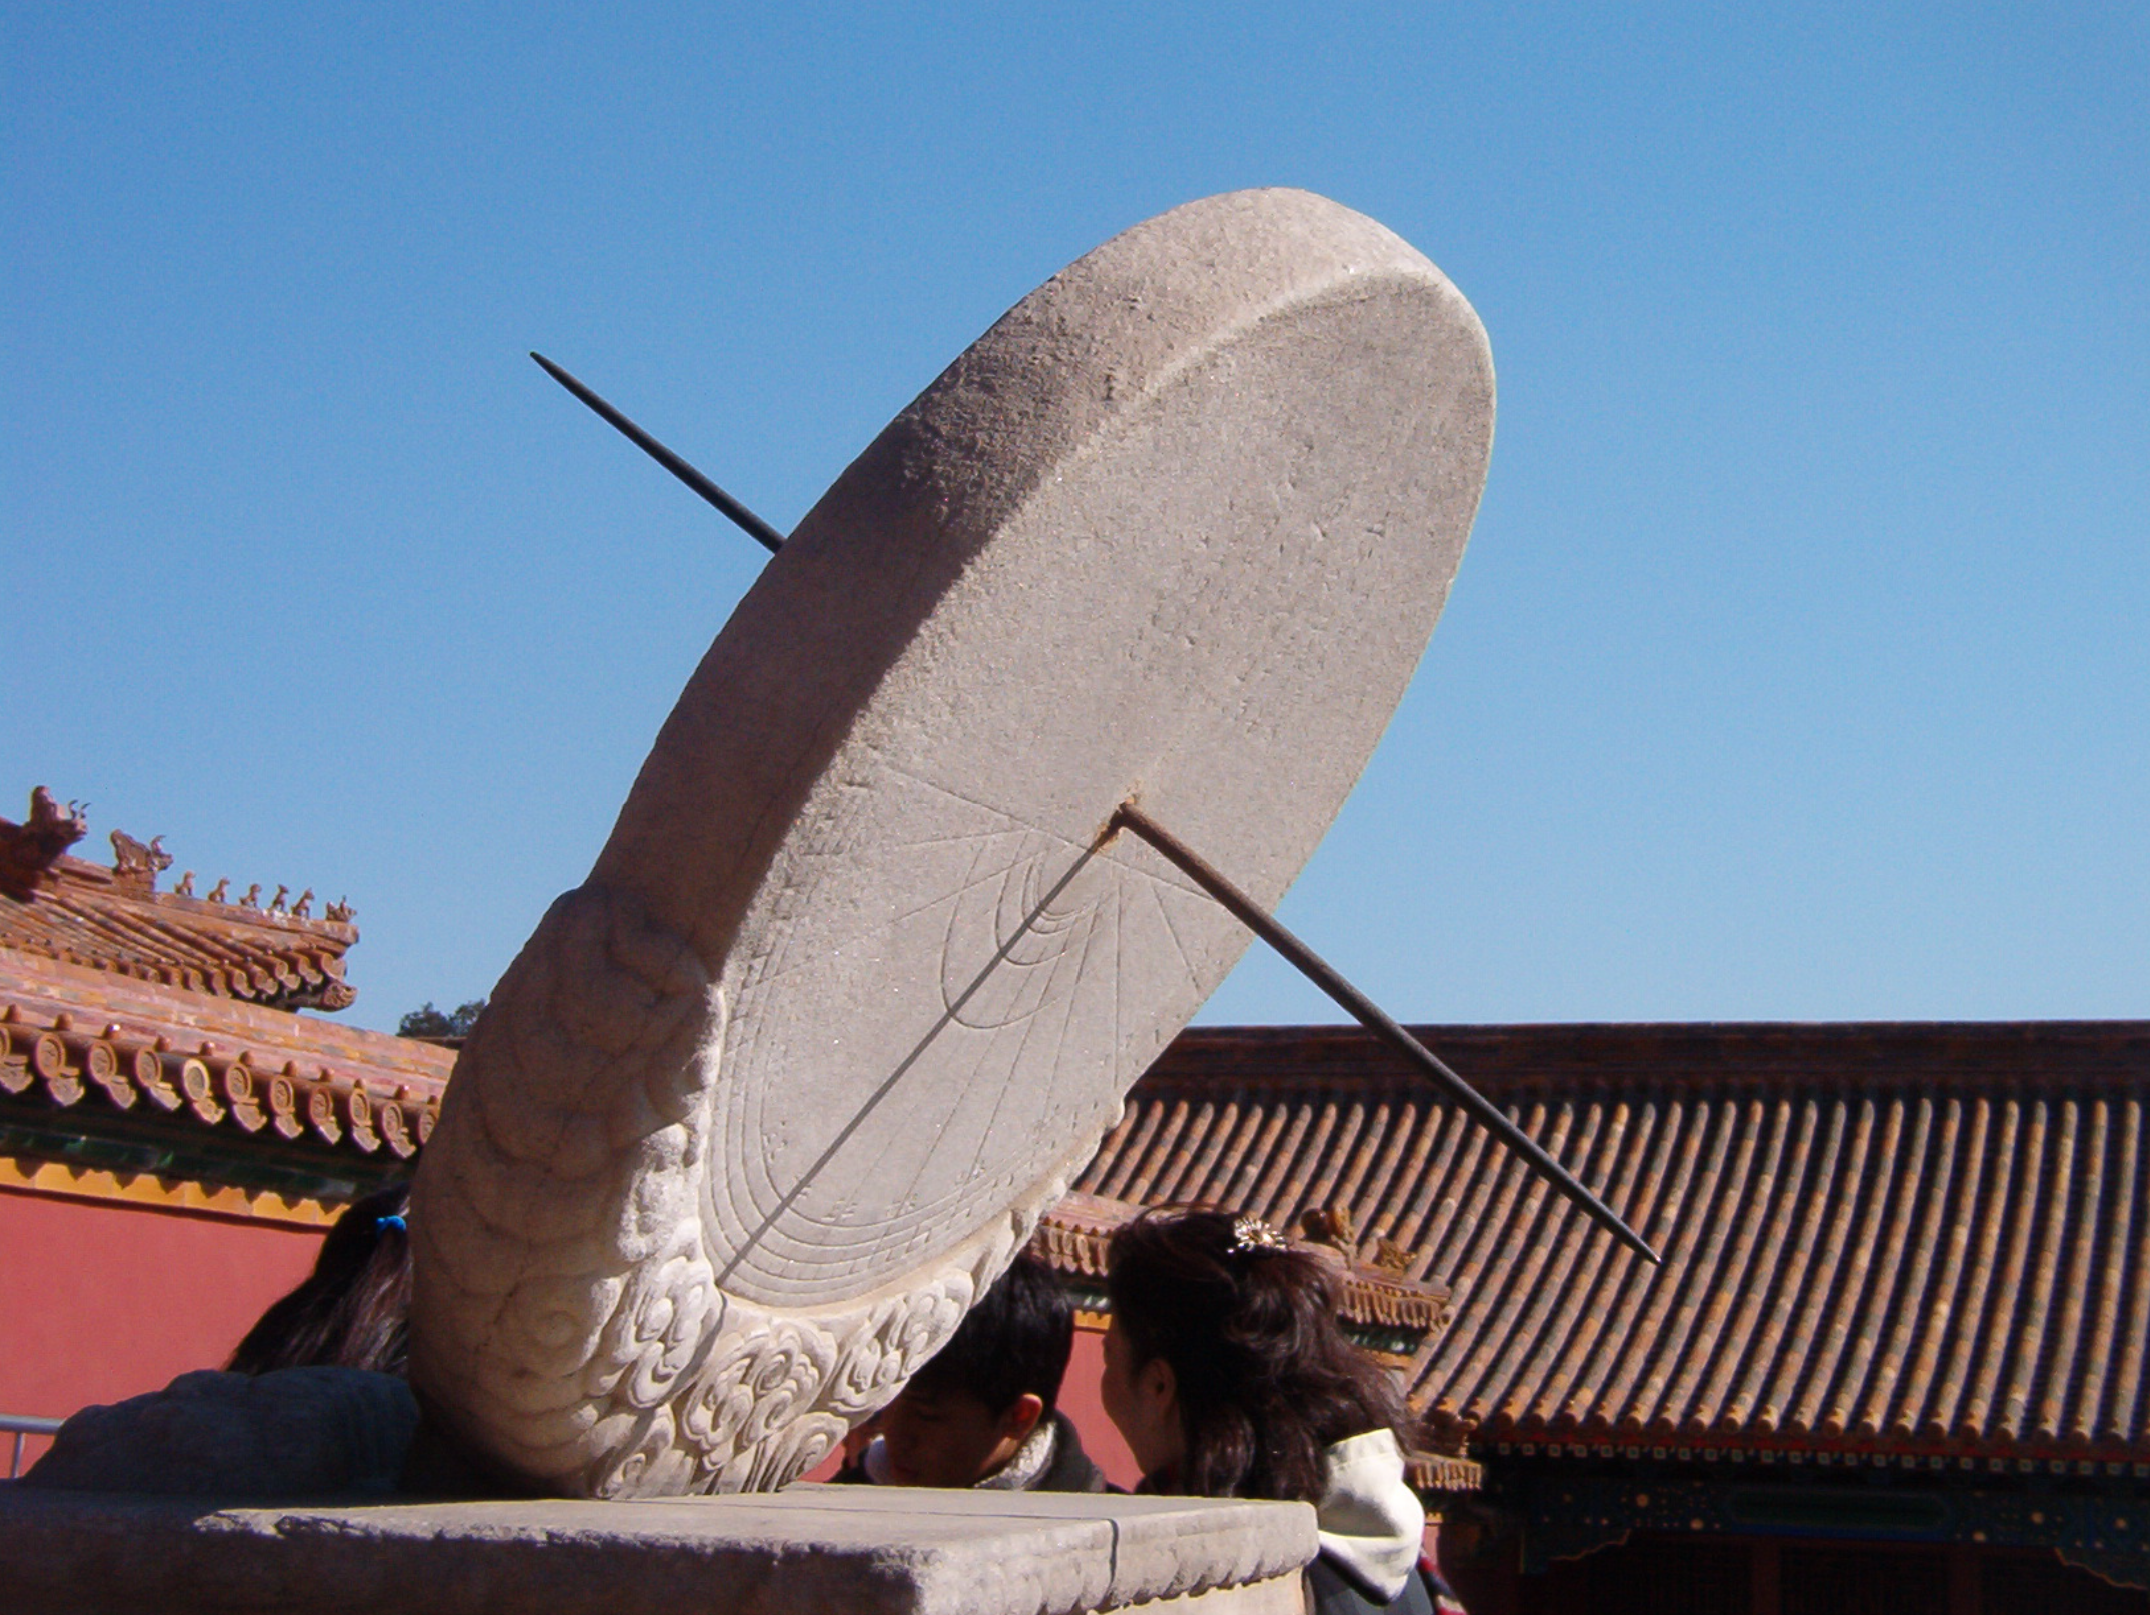
\includegraphics[width=0.5\textwidth]{EqSundial.png}
\captionsetup{labelformat=empty}
\caption{Contoh \textit{equatorial sundial}}
\label{fig:osp2022_27_jawab2}
\end{figure}

\item Andaikan papan lingkaran yang sejajar bidang ekuatorial langit ini kemudian kita ganti dengan papan vertikal, maka bentuk lingkaran akan terproyeksi menjadi bentuk elips. Di soal sebenarnya tidak terlalu jelas ``proyeksi'' yang dimaksud apakah secara tegak lurus ke dinding, atau searah dengan kemiringan bidang lingkaran (lihat ilustrasi di bawah). Definisi proyeksi benda ke suatu bidang (tanpa keterangan apapun) umumnya dengan membayangkan ada cahaya tegak lurus bidang tersebut dan bayangan yang terbentuk di bidang itulah yang kita sebut sebagai proyeksi benda di bidang (elips warna merah). Akan tetapi, melihat argumen di awal mengenai keinginan membuat \textit{vertical sundial} serta soal nomor $C$ mengenai perubahan sudut bayangan, maka sepertinya yang dimaksud soal adalah proyeksi dengan arah mengikuti kemiringan gnomon (elips warna biru).
\begin{figure}[H]
\centering
\includegraphics[width=0.65\textwidth]{osp2022_27_jawab1.png}
\captionsetup{labelformat=empty}
\caption{Proyeksi dinding mana yang dimaksud soal?}
\label{fig:osp2022_27_proj}
\end{figure}

\begin{figure}[H]
\centering
\includegraphics[width=0.55\textwidth]{sundialmath.png}
\captionsetup{labelformat=empty}
\caption{Proyeksi ke dinding vertikal untuk menghitung perubahan sudut penanda jam. Referensi: \textit{The mathematics of sundials}, Jill Vincent (2008).}
\label{fig:sundialmath}
\end{figure}

Dengan melihat geometri pada gambar di atas, panjang $b$ dapat ditentukan dengan,
\begin{eqnarray*}
    \cos{L} &=& \frac{a}{b}\\
    b &=& \frac{a}{\cos{L}} = 1,264 
\end{eqnarray*}

\item Ketika masih dalam bentuk \textit{equatorial sundial}, setiap penanda angka jam terpisah sebesar $15^{\circ}$, akan tetapi jika kita proyeksikan ke dinding vertikal, maka sudut ini berubah menyerupai transformasi elips di atas. Jika pada \textit{equatorial sundial} angka 11 tadinya berjarak $15^{\circ}$ dari angka 12, yaitu sudut POB (lihat gambar di bawah), maka pada \textit{vertical sundial} mereka akan terpisah sebesar sudut POC.
\begin{figure}[H]
\centering
\includegraphics[width=0.55\textwidth]{sundialmath2.png}
\captionsetup{labelformat=empty}
\caption{Proyeksi ke dinding vertikal untuk menghitung perubahan sudut penanda jam. Referensi: \textit{The mathematics of sundials}, Jill Vincent (2008).}
\label{fig:sundialmath2}
\end{figure}
Misalkan sudut POB = T

Panjang $\text{AB} = \text{OB} \cos{T} = a \cos{T}$ 

Panjang $\text{AO} = \text{OB} \sin{T} = a \sin{T}$

Panjang AC,
$$\text{AC} = \frac{\text{AB}}{\cos{L}} = \frac{a \cos{T}}{\cos{L}}$$

Sudut POC ($H$), sudut yang ingin kita cari sebagai proyeksi T di dinding vertikal, memiliki hubungan,
\begin{eqnarray*}
    \tan{H} &=& \frac{\text{AO}}{\text{AC}}\\
    \tan{H} &=& \frac{a \sin{T}}{\frac{a \cos{T}}{\cos{L}}}\\
    \tan{H} &=& \tan{T} \cos{L}
\end{eqnarray*}

Untuk kasus jam 11, nilai $T = 15^{\circ}$, maka sudut di dinding untuk \textit{vertical sundial}, $H = \tan^{-1}(\tan{15^{\circ}} \cos{37.7^{\circ}}) = 11,97^{\circ}$


\end{enumerate}




\vspace{0.5cm}
\question Bintang-bintang di piringan galaksi tidak hanya bergerak mengelilingi pusat Galaksi tetapi juga berosilasi terhadap bidang Galaksi. Periode osilasi bintang di piringan dapat dihitung dari rumus
$$T_\text{osilasi} = \frac{2\pi}{\sqrt{4 \pi G \rho}}$$
Dengan $\rho$ adalah rapat massa bintang di bidang Galaksi sebesar 0,1 $M_\odot$pc$^{-3}$. Untuk bintang-bintang di sekitar Matahari yang berada pada jarak $R=8$ kpc dan kecepatan bintang-bintang mengelilingi pusat Galaksi sebesar v = 220 \kms, rasio periode osilasi terhadap periode revolusi (yaitu $T_\text{osilasi}/T_\text{revolusi}$) adalah sebesar $\ldots$ 

\bigskip
\textit{Jawaban: } 0,373

Periode revolusi bintang mengelilingi galaksi,
\begin{eqnarray*}
    v &=& \frac{2 \pi R}{T}\\
    T_\text{rev} &=& \frac{2 \pi R}{v}\\
    T_\text{rev} &=& \frac{2 \pi (8000 \cdot 206265 \cdot 1,496 \times 10^8)}{220}\\
    T_\text{rev} &=& 7,05 \times 10^{15} \text{ detik} = 223,4 \text{ juta tahun}
\end{eqnarray*}
Periode osilasi bintang,
\begin{eqnarray*}
    T_\text{osi} &=& \frac{2 \pi}{\sqrt{4 \pi G \rho}}\\
    T_\text{osi} &=& \frac{2 \pi}{\sqrt{4 \pi G \left(\frac{0,1 \cdot 2 \times 10^{30}}{(206265 \cdot 1,496 \times 10^{11})^3} \right) }}\\
    T_\text{osi} &=& 2,63 \times 10^{15} \text{ detik} = 83,34 \text{ juta tahun}
\end{eqnarray*}
Nilai rasionya, $T_\text{osilasi}/T_\text{revolusi} = 0,373$


\vspace{0.5cm}
\question Gerhana Matahari hibrida akan terjadi pada tanggal 20 April 2023. Sebagian wilayah di Indonesia timur akan mengalami gerhana Matahari total, sedangkan masyarakat di daerah Micronesia akan mengalami gerhana Matahari cincin. Seandainya pada tanggal tersebut diasumsikan Bumi berada di perihelion dan Bulan berada di apogee. Diketahui eksentrisitas orbit Bumi mengelilingi Matahari adalah 0,017; eksentrisitas orbit Bulan adalah 0,055; jarak rata-rata Bumi-Matahari adalah $1,496 \times 10^8$ km; jarak rata-rata Bumi-Bulan adalah 384400; radius Matahari adalah $6,96 \times 10^5$ km; dan radius Bulan adalah 1738 km). Prosentase ukuran piringan Matahari yang akan tertutupi Bulan adalah sebesar $\ldots$ persen.

\bigskip
\textit{Jawaban: } 81.99 atau 82

Mengabaikan jari-jari Bumi, kita dapat hitung:

Jejari sudut Matahari saat Bumi di perihelion,
\begin{eqnarray*}
    \beta_\odot &=& \frac{6,96 \times 10^5}{1,496 \times 10^8 \cdot (1 - 0,017)} \text{  rad}\\
    &=& 4,732865 \times 10^{-3} \text{  rad}\\ 
    &=& 16,2704 \text{ menit busur}
\end{eqnarray*}
Jejari sudut Bulan saat ia di apogee,
\begin{eqnarray*}
    \beta_{\leftmoon} &=& \frac{1738}{384400 \cdot(1 + 0,055)} \text{  rad}\\
    &=& 4,2856227 \times 10^{-3} \text{  rad}\\
    &=& 14,7329 \text{ menit busur}
\end{eqnarray*}
Rasio piringan Matahari yang akan tertutupi bulan
\begin{eqnarray*}
    \frac{14,7329^2}{16,2704^2} \times 100\% = 81,99\%
\end{eqnarray*}

\vspace{0.5cm}
\question Diketahui awan antar galaksi menyebabkan garis absorpsi Lyman-alpha 1215 \AA dengan pelebaran Doppler sebesar 29,6 \kms. Berapakah temperatur awan tersebut dalam satuan Kelvin? Gunakan besaran massa atom Hidrogen $=1,6735575 \times 10^{-27}$ kg dan konstanta Boltzmann $=1,38 \times 10^{-23}$ m$^2$ kg s$^{-1}$ K$^{-1}$

\bigskip
\textit{Jawaban: } 53127 K 

\textit{Kunci: } 53000 (toleransi 53000-53110) K

Pelebaran Doppler diakibatkan oleh gerak acak partikel di dalam gas. Jika kita anggap awan Hidrogen ini merupakan gas ideal, maka distribusi kecepatannya akan  mengikuti bentuk distribusi Maxwell-Boltzmann dengan nilai kecepatan partikel di dalamnya terbanyak sebesar,
\begin{eqnarray*}
    v_\text{most probable} &=& \sqrt{\frac{2 k T}{ m}}\\
    T &=& \frac{v_\text{most probable}^2 \cdot m}{2 k}\\
    T &=& \frac{29600^2 \cdot 1,6735575 \times 10^{-27}}{2 \cdot 1,38 \times 10^{-23}}\\
    T &=& 53127 \text{ K}
\end{eqnarray*}
Referensi: \url{https://jila.colorado.edu/~pja/astr3730/lecture09.pdf}


\end{questions}

% \vspace{0.5cm}
% \question Dalam
% \begin{choices}
% \choice Rata-rata
% \choice Median
% \choice Modus
% \choice Standar Deviasi
% \choice Variansi
% \end{choices}

% \bigskip
% \textit{Jawaban: } B

%\centering{\--- SOAL SELESAI\---}

\vspace{3cm}
\begin{flushright}
%Hitungan lebih detail bisa di cek di \url{https://s.id/HitunganOSP2020}\\
Solusi seperti ini dapat diperoleh di \url{http://ridlow.wordpress.com}
\end{flushright}


\end{document}